\setcounter{ExampleCounter}{1}
\begin{center}

\includegraphics[width=0.8\textwidth]{cottage}
\end{center}

When the time comes to buy a home, you'll need to start shopping around for a \textbf{mortgage}, which is a long-term loan that is secured against whatever home you purchase.  What this means is that if you fail to make your payments and \emph{default} on your loan, the bank can \emph{foreclose} on your house and take it from you in order to pay your debt.  In this section you'll learn how to plan for buying a home.

\subsection{Mortgage Concepts}
Before we start doing calculations with specific formulas, we should discuss some of the terminology related to mortgages.  There are plenty of terms we won't discuss here, but this should be enough to get started.\\

First, a mortgage is an example of an \textbf{installment loan}, which is a loan that is paid off in installments, meaning that you receive a lump sum when you take out the loan, and you pay this loan back in regular monthly payments.  Installment loans are not unique to mortgages; this also describes car payments, for instance, so we'll start with examples about buying a car.\\

Next, you cannot borrow the full amount needed to purchase a home; for a large loan like this, you need to pay a \textbf{down payment} up front.  The reason for this is simple: if none of your own money is tied up in the home, the bank is the one taking all the risk, so you need to come up with part of the money, and from their perspective this investment is your incentive to not default on the loan.  Typical down payments range from 10\% to 20\% of the price of the home.  There are exceptions, like FHA loans, which are guaranteed by the Federal Housing Administration; with these, you can put down as little as 3.5\%.  As we will see, though, it is in your best interest to save up as much as you can for the down payment, especially since a down payment lower than 20\% requires \textbf{mortgage insurance}, which is a fee added to your monthly payment that pays for insurance against the bank's investment.  This insurance will automatically drop off eventually, once you own at least 20\% of the home.\\

The life of a mortgage can vary, but the most typical mortgages are structured for 30 years.  Fifteen-year and 20-year mortgages are also fairly common; the faster you pay back the loan, the less you'll end up paying overall, but the trade-off is that your monthly payments will be higher (we'll see examples of this in this section).  Mortgages can be \textbf{fixed-rate} or \textbf{adjustable-rate}.  As the name implies, the interest rate can change for an adjustable-rate mortgage; the bank will recalculate the rate based on the current market.  You may hear of a mortgage like a 5/1 ARM; this is an adjustable-rate mortgage (ARM) in which the rate is fixed for the first 5 years, and then every year after that, it is recalculated.\\

There are other costs in addition to simply paying back the loan, and we'll account for a few of them in this section.  For instance, when you initiate a mortgage, there are one-time \textbf{closing costs}, which include things like taxes, fees to the lender and title company, land surveys, inspections, and so on.  This just means that when you get ready to buy a home, you need to plan to have your down payment plus the closing costs on hand.
\pagebreak

In addition to the loan payment (often referred to as \emph{principal and interest} or \emph{P\&I}), a few other payments are added each month; the two most common are property taxes and homeowner's insurance.  This is largely for convenience; rather than having to plan for a large insurance or tax payment at the end of the year, those get bundled into your mortgage payment so that you can easily budget for it all each month.  The way this works is that the bank handles making the tax and insurance payments at the end of the year for you.  Throughout the year, as the bank collects your mortgage payment, they set aside the portion of it that corresponds to taxes and insurance and place that into what is called an \textbf{escrow} account.  Then at the end of the year, the bank automatically withdraws the right amount from the escrow account and pays the bills.

\begin{formula}{Summary: Mortgage Terminology}
\paragraph{Installment Loan:} A loan that is paid off in regular (usually monthly) payments.

\paragraph{Down Payment:} A portion of the cost of a home (or car, etc.) that is paid up front; the loan covers the rest of the cost.

\paragraph{Mortgage Insurance:} If a homebuyer puts down less than 20\% of the cost, they must purchase insurance against defaulting.

\paragraph{Closing Costs:} One-time fees that are paid at the time of purchase; these do not go toward the cost of the home.

\paragraph{Escrow:} An account used to hold the portion of the mortgage payment designated for taxes and insurance.
\end{formula}

That's a lot of information all at once, but it's important to understand these terms, because we will use them in the examples in this section.

\subsection{Installment Loan Formula}
At the core of the problems we'll be doing a bit later is the calculation of the loan payment, which is sometimes called P\&I.  This means that this payment is used to slowly pay down the principal of the loan, but it also must pay for the interest that the loan is accruing even as it is being paid off.

This may sound complicated now, but toward the end of the section, we'll break down exactly how a payment is divided between principal and interest, using \emph{amortization tables}.

\paragraph{Calculating the payment on an installment loan:} It turns out that we've actually seen this formula before: it's the one for finding the payment amount for a payout annuity.\\

To see this, imagine that you had \$5000 invested at a bank and you started taking out payments while earning interest (a payout annuity), and after 5 years your balance was zero.  Now flip that around and put yourself in the position of a bank: now the lender is investing \$5000 in you (you take a loan of \$5000) and you start to pay them back in equal payments as the remaining balance earns interest, and after 5 years the balance is zero.\\

Since we're generally interested in finding the payment amount (we usually start by knowing how much we need to borrow), we'll use the version of the payout annuity formula that is solved for $PMT$, but if you want to start with what monthly payment you can afford and find out how much you can borrow, you can rearrange this formula, or simply refer to the version that we mainly used with payout annuities.\\

\begin{formula}{Installment Loan Payment}
If an installment loan of $P$ is taken out at an interest rate of $r$ compounded $n$ times a year, and paid back in equal payments $n$ times a year over $t$ years, the payment amount $PMT$ is given by
\[PMT = \dfrac{P\left(\dfrac{r}{n}\right)}{1-\left(1+\dfrac{r}{n}\right)^{-nt}}\]
\end{formula}

Let's do a few examples, starting with car loans, since that way we don't have to worry about escrow accounts and closing costs just yet.

\begin{example}[https://www.youtube.com/watch?v=RVUWTbil3fQ]{Car Loan}
If you take out an auto loan of \$11,000 at 4\% interest for 60 months, what will your monthly payment be?\\

\sol
Notice that we haven't mentioned a down payment here, but you are probably (hopefully) not borrowing the full cost of the car.  Many car dealers will offer 0\% down loans, but it is in your best interest to only borrow what you have to, not as much as they will offer you.

Start by organizing the given information:
\begin{center}
\begin{tabular}{r l l}
$P$ & \$11,000 & The loan amount\\
$r$ & 0.04 & 4\% interest rate\\
$n$ & 12 & Payments made monthly\\
$t$ & 5 & 60 months = 5 years
\end{tabular}
\end{center}

Simply use the formula:
\begin{align*}
PMT &= \dfrac{\$11,000\left(\dfrac{0.04}{12}\right)}{1-\left(1+\dfrac{0.04}{12}\right)^{-(12)(5)}}\\
&= \boxed{\$202.58}
\end{align*}
Thus you'll end up paying \$202.58 every month for five years.
\end{example}

\begin{try}[http://izzomath.com/103text/finance/example5.1/story.html]
If you take out an auto loan of \$15,000 at 5.6\% interest for 72 months, what will your monthly payment be?
\end{try}

Now let's flip the question around: if you can budget for a car payment, how much of a loan can you afford?

\paragraph{Note:} there's a common pitfall here.  Depending on what salesperson you talk to, they may attempt to start with this question.  The reason is that it's easy for you to imagine spending \$50 more each month, but if they told you how much of a total difference that makes up front, the number would be much more intimidating.  You should always run your own calculations to check things like how much the total cost will change, and how much the total interest charge would change over time.
\pagebreak

\begin{example}[https://www.youtube.com/watch?v=ydmN5lt5g20]{How Much Can You Afford?}
You can afford a monthly car payment of \$250.  If you find a bank offering 4.85\% interest on a 60 month loan, what is the largest car loan you can afford?\\

\sol
In this case $PMT$ is known and $P$ is the unknown that we want to find:
\begin{center}
\begin{tabular}{r l l}
$PMT$ & \$250 & The loan amount\\
$r$ & 0.0485 & 4.85\% interest rate\\
$n$ & 12 & Payments made monthly\\
$t$ & 5 & 60 months = 5 years
\end{tabular}
\end{center}

Now use the formula and solve for $P$:
\begin{align*}
\$250 &= \dfrac{P\left(\dfrac{0.0485}{12}\right)}{1-\left(1+\dfrac{0.0485}{12}\right)^{-(12)(5)}}\\
\$250 &= P(0.0188)\\
\boxed{\$13,296} &\approx P
\end{align*}
You can afford a car loan of \$13,296 under these terms; of course, this is the maximum you can afford, so it wouldn't hurt to take out a smaller loan that this if you can.
\end{example}

\begin{try}[http://izzomath.com/103text/finance/example5.2/story.html]
You can afford a monthly car payment of \$300.  If you find a bank offering 6.7\% interest on a 48 month loan, what is the largest car loan you can afford?
\end{try}

\begin{example}[https://www.youtube.com/watch?v=rhTeMJm8-Lc]{Actual Cost}
You see a TV ad that says ``We can put you in the car of your dreams!!! Drive this brand-new \$25,000 car off the lot with only \$500 down and a monthly payment of \$550 for 60 months.''  How much do you end up actually paying for the car?\\

\solline
\marginnote{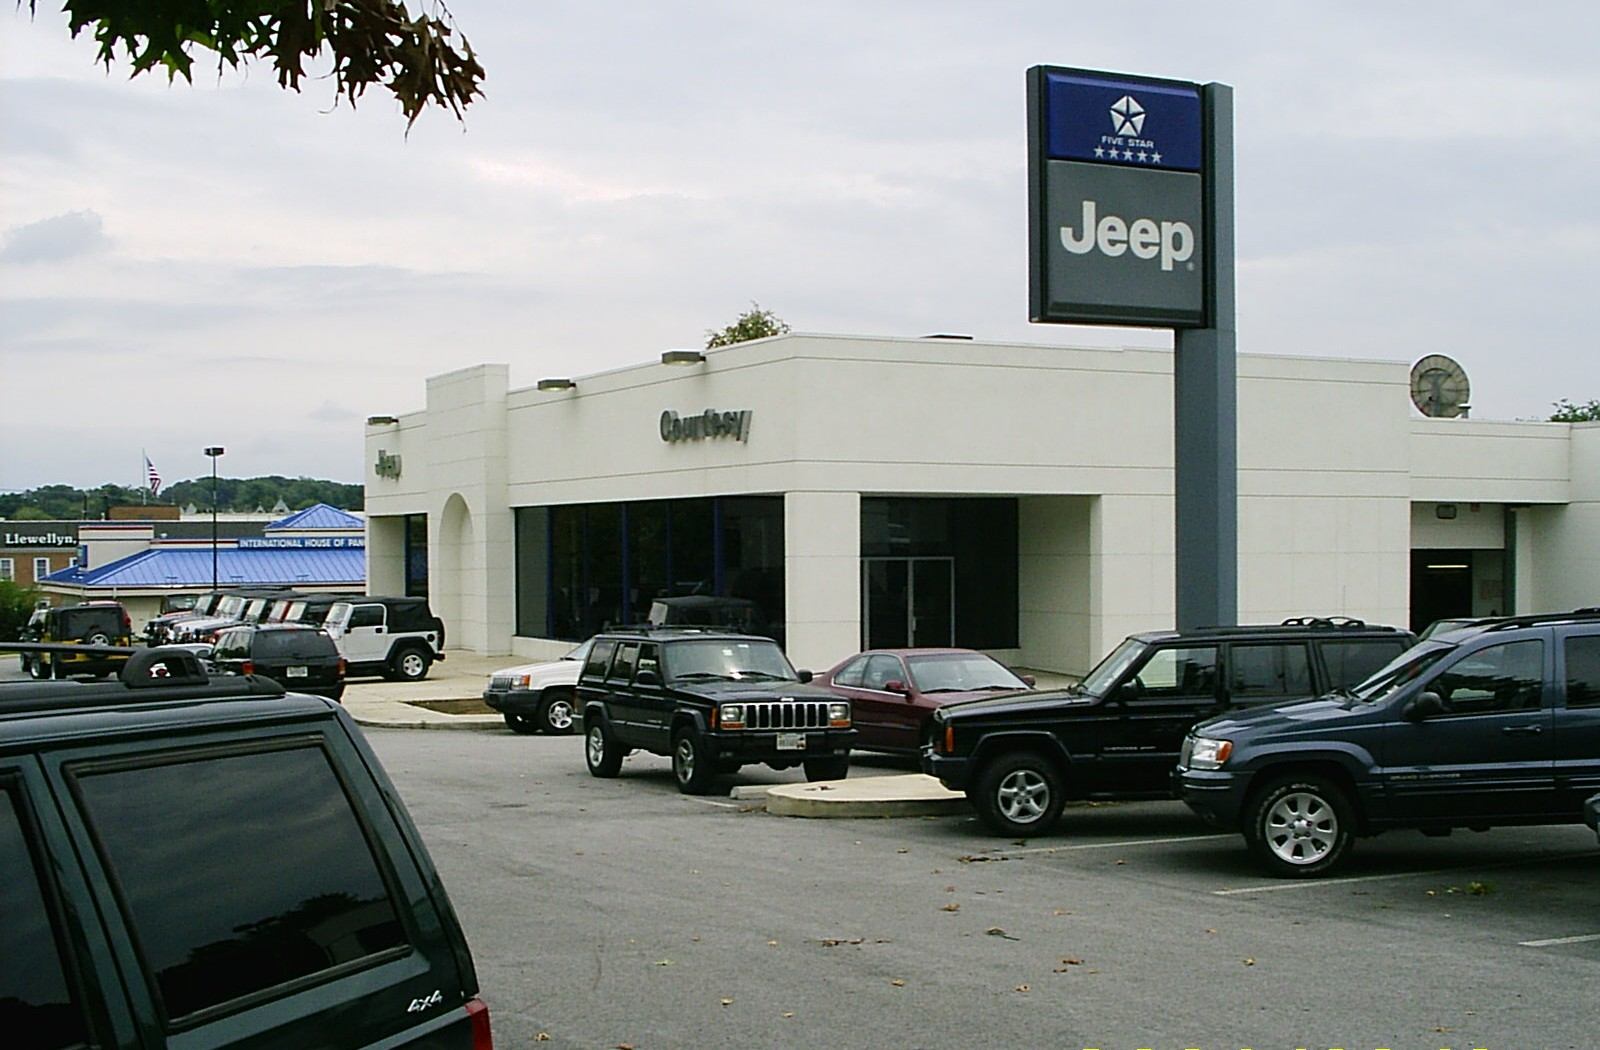
\includegraphics[scale=0.06]{CarDealer1}}
First, let's find out how much the car actually costs you.

The down payment is the amount that is due at the beginning, so if we add that to 60 payments of \$550, we'll have the total amount that comes out of your pocket:
\[\$500 + (60)(\$550) = \$33,500\]

This means that you pay \$33,500 for a \$25,000 car, and the difference is the interest on the loan:\marginnote{\footnotesize\textcolor{black!60}{Photo by Christopher Ziemnowicz}}
\[\$33,500 - \$25,000 = \boxed{\$8500}\]

Are you really willing to pay \$8500 in interest to have the car now, or can you save up first and pay for it in cash---at least in part---to reduce this interest cost?
\end{example}

\begin{try}[http://izzomath.com/103text/finance/example5.3/story.html]
A boat costs \$12,000, and you're offered a loan that requires \$1000 down and \$250 a month for 60 months.  Find the total amount you would pay for the boat and the amount of interest you would pay with this loan.
\end{try}

This example emphasizes an important point: when you're offered a loan, don't focus on the monthly payment; instead, calculate the total cost of the loan and decide if it is worth it to you.
\vfill
\pagebreak

\subsection{Mortgage Example}
If you need to, you can review the terminology introduced at the beginning of the section, because we'll be using those terms in the following examples.

\paragraph{Fair warning:} The next example is a long one, because it includes all the components we discussed at the beginning of the section.  The good news is that this is a pretty realistic example, so if you can understand this, you'll be well prepared for the real thing.

\begin{example}{Buying a Condo}
\marginnote{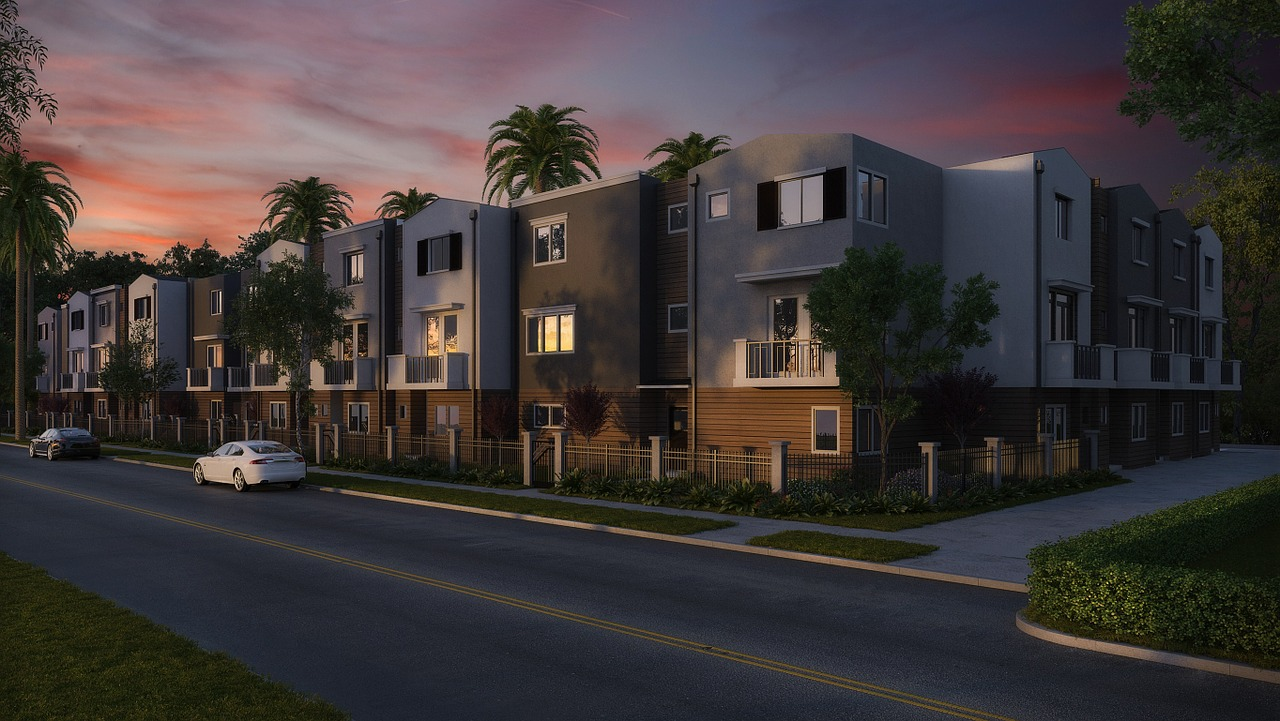
\includegraphics[width=1.5in]{Condo1}}
The price of a condominium is \$180,000, and your bank offers a 30-year fixed mortgage at 4\% interest.  You have \$32,000 available right now.
\begin{enumerate}[(a)]
\item Your banker tells you to expect \$5000 in closing costs.  What percentage down payment can you afford?  Will you need mortgage insurance?
\item What will the principal be on the mortgage?
\item What will your monthly P\&I payment be?
\item In addition to principal and interest, your monthly payment will need to account for property taxes, homeowners insurance, and mortgage insurance, if necessary (find out in part (a)):
\begin{center}
\begin{tabular}{l r}
\textbf{Property Taxes:} & 1.5\% of the home value per year\\
\textbf{Homeowners Insurance:} & \$900 per year\\
\textbf{Mortgage Insurance:} & \$40 per month
\end{tabular}
\end{center}
What will your total monthly payment amount be?
\item How much will you pay in total over 30 years in principal and interest?
\item How much interest will you pay in total?
\end{enumerate}

\sol
There's a lot here, but if we take it one part at a time, the actual calculations are fairly simple.

\begin{enumerate}[(a)]
\item Down payment and mortgage insurance:

Since you need to set aside \$5000 for closing costs, this leaves \[\$32,000 - \$5000 = \$27,000\] for a down payment.  To find what percentage this represents of \$180,000, divide the down payment by the total cost:
\[\dfrac{\$27,000}{\$180,000} = 0.15 = 15\%\]

Therefore, you can afford a down payment of $\boxed{15\%}$, so \textbf{yes, you must pay for mortgage insurance}.

\item Mortgage principal:

The principal on the mortgage is the amount you need to borrow, or the difference between the cost of the home and the down payment, the portion that you can pay in cash.  Since the down payment will be \$27,000,
\begin{align*}
\textrm{Principal } &= \$180,000 - \$27,000\\
&= \boxed{\$153,000}
\end{align*}

\item Monthly principal and interest payment ($PMT$):

This is where we actually have to pull out a complicated formula:
\[PMT = \dfrac{P\left(\dfrac{r}{n}\right)}{1-\left(1+\dfrac{r}{n}\right)^{-nt}}\]

We know that $P$, the principal, will be \$153,000, the interest rate is 4\% (0.04), and $t$ is 30 years, so we can calculate $PMT$:
\begin{align*}
PMT &= \dfrac{\$153,000\left(\dfrac{0.04}{12}\right)}{1-\left(1+\dfrac{0.04}{12}\right)^{-(12)(30)}}\\
&= \boxed{\$730.45}
\end{align*}

This is the amount we'll pay each month just on the loan, but the next part will add to it to give our total payment amount, including the escrow and mortgage insurance (remember, we \textbf{do} require mortgage insurance in this example, but that will not be true in examples where the down payment is at least 20\%).

\item Total monthly payment:

Starting with the P\&I amount of \$730.45, we also need to add taxes, homeowners insurance, and mortgage insurance.  Start by calculating the monthly cost of each component (divide the yearly cost by 12):
{\small
\begin{center}
\begin{tabular}{l r r}
\textbf{P\&I:} & & \$730.45 per month\\
\textbf{Property Taxes:} & Yearly: $(1.5\%)(\$180,000) = \$2700$ & \$225 per month\\
\textbf{Home Insurance:} & \$900 per year & \$75 per month\\
\textbf{Mortgage Insurance:} & & \$40 per month
\end{tabular}
\end{center}}

Adding them all together:
\begin{align*}
\textrm{Monthly Payment } &= \textrm{ P\&I } + \textrm{ Property Tax }\\
&+ \textrm{ Home Insurance } + \textrm{ Mortgage Insurance }\\
&= \$730.45 + \$225 + \$75 + \$40\\
&= \boxed{\$1070.45}
\end{align*}

The final amount you can expect to pay each month is \$1070.45.

\item Total principal and interest paid:

It's easy to calculate how much you will pay in total for the loan: simply multiply your monthly P\&I payment by the number of payments you will make (12 payments a year for 30 years is $(12)(30) = 360$ payments).  Note that the tax and insurance payments are not involved here; we're simply looking for the total principal and interest paid:
\[(\$730.45)(360) = \boxed{\$262,962}\]

Over 30 years, you'll pay a total of \$262,962 for this condo, including the loan interest.

\item Total interest paid:

Now that we know how much you'll pay in principal \emph{and} interest (from the last part), and we know what the principal on the loan is (part (b)), we can subtract to isolate the interest:

\[\$262,962 - \$153,000 = \boxed{\$109,962}\]

Notice that we didn't subtract the total cost of the condo, only the amount that we had to borrow from the bank (we don't pay interest on the amount covered by the down payment).
\end{enumerate}
\end{example}

\begin{try}
The price of a home is \$340,000, and your bank offers a 30-year mortgage at 3.5\% interest.  You have \$60,000 available right now, and the banker tells you to expect \$8000 in closing costs.  Complete parts (a) - (f) of the previous example, using the same values for taxes and insurance.
\end{try}
\pagebreak

\subsection{Changing the Loan Terms}
Let's take a look now at what happens if we change the terms of the loan.  To begin, we'll set up a baseline using a 30-year fixed-rate loan at 4\% and assume that we're borrowing \$200,000.  We won't need to account for a down payment, closing costs, or escrow, since we're only focused on the loan itself for the time being.

Then we'll see what happens if 
\begin{enumerate}[(a)]
\item the interest rate changes,
\item the loan amount changes (if, for instance, we made a larger down payment),
\item or the length of the loan changes.
\end{enumerate}

To make these comparisons, we'll use the same measurement each time: the total interest paid over the life of the loan.  This is a good number to track, because it gives a sense of how much the loan costs (the principal must be paid back no matter what, but by altering the terms, we can alter the amount of interest).\\

We won't show the details of the calculations here, in order to focus on the results.  If you like, you can refer to the description of using the TVM solver with payout annuities to follow along with the calculations quickly.

\begin{example}{Changing the Interest Rate}
Compare a 30-year fixed-rate loan at 4\% for \$200,000 to the same loan at 3.5\% by finding the total amount paid in interest for both versions.

\sol
To compare the total interest paid in each case, we need to find the monthly payment for each, then multiply this by the number of payments (360 for a 30-year loan) and subtract the principal of the loan (\$200,000):
\begin{center}
\begin{tabular}{r c c}
& \textbf{4\%} & \textbf{3.5\%}\\
\textbf{Monthly payment:} & \$954.83 & \$898.09\\
\textbf{Total paid:} & \$343,738.80 & \$323,312.40\\
\textbf{Interest paid:} & $\boxed{\$143,738.80}$ & $\boxed{\$123,312.40}$
\end{tabular}
\end{center}

By reducing the interest rate by just half of one percentage point, you could save over \$20,000 over time (not to mention that if you invested the \$56.74 that you save each month at 7\%, you could save up nearly \$70,000 over the same time).
\end{example}

\begin{example}{Changing the Loan Amount}
Compare a 30-year fixed-rate loan at 4\% for \$200,000 to the same loan for \$180,000 by finding the total amount paid in interest for both versions.

\sol
We can copy the values from the previous example for the baseline loan, so we only need to calculate the monthly payment and other values for the reduced loan:
\begin{center}
\begin{tabular}{r c c}
& \textbf{\$200,000} & \textbf{\$180,000}\\
\textbf{Monthly payment:} & \$954.83 & \$859.35\\
\textbf{Total paid:} & \$343,738.80 & \$309,366.00\\
\textbf{Interest paid:} & $\boxed{\$143,738.80}$ & $\boxed{\$129,366.00}$
\end{tabular}
\end{center}

In this case, you could save over \$34,000 in total by paying \$20,000 more up front or finding a less-expensive home (or some combination of the two).  Of that, about \$14,000 is the amount saved on interest alone.
\end{example}
\pagebreak

\begin{example}{Changing the Length of the Loan}
Compare a 30-year fixed-rate loan at 4\% for \$200,000 to the same loan for 20 years and for 15 years by finding the total amount paid in interest for all three versions.

\sol
Again, the baseline loan will have the same values as always, and we will only change the length of the loan in the other two cases (note that to calculate the total paid, we multiply the 20-year monthly payment by 240, and we multiply by 180 for the 15-year loan):
\begin{center}
\begin{tabular}{r c c c}
& \textbf{30 years} & \textbf{20 years} & \textbf{15 years}\\
\textbf{Monthly payment:} & \$954.83 & \$1211.96 & \$1479.38\\
\textbf{Total paid:} & \$343,738.80 & \$290,870.40 & \$266,288.40\\
\textbf{Interest paid:} & $\boxed{\$143,738.80}$ & $\boxed{\$90,870.40}$ & $\boxed{\$66,288.40}$
\end{tabular}
\end{center}

Notice the trade-off here: shorter loans require higher monthly payments, because you have to pay down the loan faster, but the end result is that you pay much less in interest overall (a total of over \$77,000 in the most extreme case).  Of course, this all depends on the budget that you can work with.
\end{example}

You could, of course, experiment with changing all three factors at once, but at least these examples give us a sense of the total cost of a loan can change dramatically by adjusting the terms of the loan.  When you start shopping for a mortgage, these are all factors to keep in mind.

\subsection{Amortization Tables}
When you take out a mortgage, you'll receive in your loan packet a long table with hundreds of rows, and it's easy for your eyes to glaze over as you scan the columns of numbers marching down, but we're going to see that an \textbf{amortization table} is actually quite simple to understand.

The concept is this: we've used the term P\&I (principal and interest) to describe the payment you make to the bank to pay back the loan.  Each month, the balance that you currently own accrues interest, and part of your payment goes to pay off that interest.  Whatever is left over after paying interest is used to pay down the balance.

This means that as time goes on, and the balance slowly drops, the amount you owe in interest each month decreases as well, so more of your monthly payment can be used to pay down the balance, driving it down even faster, and the process accelerates.

In practice, you'll notice that at the beginning of the process, a lot of your payment goes toward interest, but later in the life of the loan, the balance will shift, and the majority of your payment will go toward principal.  The formula used to calculate your monthly payment ensures that at the end of the process, the balance drops to 0 exactly.

Here's a visual of what it looks like:
\begin{center}
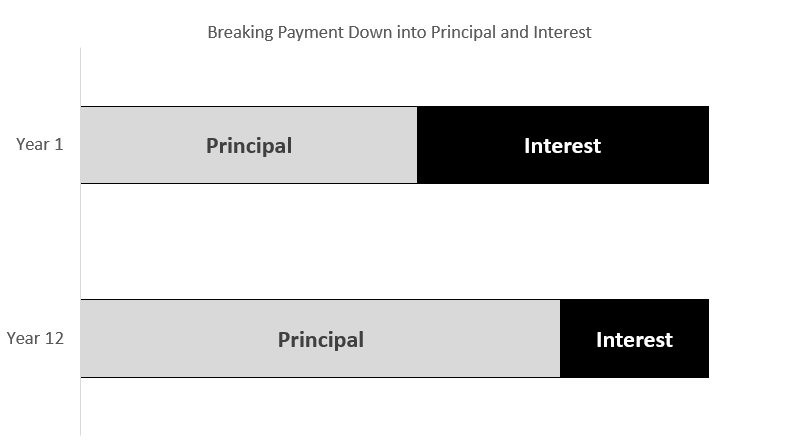
\includegraphics[width=0.8\textwidth]{AmortizationBreakdown}
\end{center}
In year 1, the payment is about evenly split between principal and interest, but by year 12, the overwhelming majority goes to principal (this example was taken from a 20-year mortgage).

Notice that the overall payment never changes; it's just that the line separating the principal from the interest shifts slowly to the right over time.  The final payment of the loan will pay just pennies in interest.

\begin{formula}{Amortization Table}
An \textbf{amortization table} lists the payments of an installment loan in order, showing the amount of each payment that goes toward interest and the amount that goes to toward principal.\\

An amortization table will typically have four columns: the payment number, the interest for that payment, the amount of that payment that goes toward principal, and the remaining balance after the payment.

\begin{center}
\begin{tabular}{|c | c | c | c|}
\hline
Payment Number & Interest Payment & Principal Payment & Loan Balance\\
\hline
& & &
\end{tabular}
\end{center}
\end{formula}

The calculations needed to build an amortization table are very simple, but repetitive, so we'll only build a few rows by hand, and we'll use Excel if we want a full table.

After building a table, you should notice that as you scan down the table, the interest payments decrease, the principal payments increase, and the balance slowly drops.\\

Let's see an example of building a table like this.

\begin{example}[https://www.youtube.com/watch?v=bgFXXvgNB0g]{Loan Amortization Schedule}
Suppose you take out a 20-year mortgage for \$200,000 at 7\% interest, with monthly payments of \$1550.60 (we know how to calculate this now, but it is given to us to simplify this example).  Prepare an amortization schedule for this loan.

\sol
Only one calculation is really needed at each stage---calculating the interest due for that month (everything else follows from that).  To calculate the interest due for a particular month, use the simple interest formula ($I=Prt$); since we're only looking at one payment period, there's no compounding happening.  The principal $P$ will be the loan balance at that point, $r$ is the same for every payment, and $t$ will be 1/12, since we're dealing with a month, a twelfth of a year.
\begin{enumerate}
\item The first payment:
\begin{align*}
\textrm{Interest } &= Prt = (\$200,000)(0.07)\left(\dfrac{1}{12}\right) = \$1166.67\\
\textrm{Principal Payment } &= \textrm{ Monthly Payment } - \textrm{ Interest}\\
&= \$1550.60 - \$1166.67 = \$383.93\\
\textrm{Balance } &= \textrm{ Previous Balance } - \textrm{ Principal Payment}\\
&= \$200,000 - \$383.93 = \$199,616.07
\end{align*}

\item The second payment: the starting balance for the second month is the final balance at the end of the first month, \$199,616.07.
\begin{align*}
\textrm{Interest } &= Prt = (\$199,616.07)(0.07)\left(\dfrac{1}{12}\right) = \$1164.43\\
\textrm{Principal Payment } &=  \$1550.60 - \$1164.43 = \$386.17\\
\textrm{Balance } &= \$199,616.07 - \$386.17 = \$199,229.90
\end{align*}
\end{enumerate}
To fill out the rest of the table, we could continue these calculations until we've covered all 240 payments, but of course this is far too tedious to do by hand, so we have a computer do it for us.  The table below shows a few of the payments, skipping through to show payments at various stages of the loan.
\begin{center}
\begin{tabular}{|>{\centering\arraybackslash\hspace{0pt}}p{1in} | >{\centering\arraybackslash\hspace{0pt}}p{1in} | >{\centering\arraybackslash\hspace{0pt}}p{1.1in} | >{\centering\arraybackslash\hspace{0pt}}p{1in}|}
\hline
{\small Payment Number} & {\small Interest Payment} & {\small Principal Payment} & {\small Balance of Loan}\\
\hline
1 & 1166.67 & 383.93 & 199616.07\\
\hline
2 & 1164.43 & 386.17 & 199229.90\\
\hline
3 & 1162.17 & 388.42 & 198841.47\\
\hline
4 & 1159.91 & 390.69 & 198450.79\\
\hline
\vdots & \vdots & \vdots & \vdots\\
\hline
30 & 1096.12 & 454.47 & 187452.64\\
\hline
31 & 1093.47 & 457.12 & 186995.52\\
\hline
\vdots & \vdots & \vdots & \vdots\\
\hline
145 & 663.44 & 887.16 & 112845.43\\
\hline
146 & 658.26 & 892.33 & 111953.09\\
\hline
\vdots & \vdots & \vdots & \vdots\\
\hline
239 & 17.93 & 1532.66 & 1541.61\\
\hline
240 & 8.99 & 1541.61 & 0.00\\
\hline
\end{tabular}
\end{center}

This illustrates the key features of an amortization table:
\begin{itemize}
\item The interest payment and principal payment in each row add up to the same monthly payment.
\item The balance of the loan slowly shrinks and goes exactly to zero with the last payment.
\item The amount of the payment that goes to interest shrinks each month and the amount that goes to paying down the principal grows by an equal amount.
\end{itemize}
\end{example}

\begin{try}[http://izzomath.com/103text/finance/example5.6/story.html]
If you take out a loan for \$175,000 at 4.5\% interest for 30 years, with a monthly payment of \$886.70, find values for A-F that will correctly fill out the first two rows of the amortization table below.
\begin{center}
\begin{tabular}{|>{\centering\arraybackslash\hspace{0pt}}p{1in} | >{\centering\arraybackslash\hspace{0pt}}p{1in} | >{\centering\arraybackslash\hspace{0pt}}p{1in} | >{\centering\arraybackslash\hspace{0pt}}p{1in}|}
\hline
{\small Payment Number} & {\small Interest Payment} & {\small Principal Payment} & {\small Balance of Loan}\\
\hline
1 & A & B & C\\
\hline
2 & D & E & F\\
\hline
& & &
\end{tabular}
\end{center}
\end{try}
\vfill
\pagebreak

\subsection{Using Excel to Create Amortization Tables}
Again, we would never build a full amortization table by hand, but we can use a spreadsheet program to simplify the process.  To begin, open Excel and enter the details of a loan, as shown.  If we use these values to calculate the rest of the table, we can change any of the terms of the loan and watch the table update immediately for easy comparison.
\begin{center}
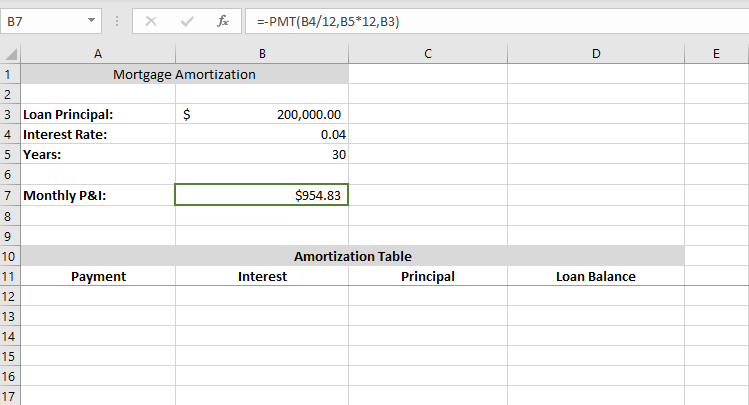
\includegraphics[width=0.75\textwidth]{ExcelAmortizationSetup}
\end{center}

Notice that to calculate the monthly payment, we're using the formula for PMT, as shown in the section on Saving for Retirement.

The key to avoid lots of typing is that you can select a cell or group of cells and drag downward from there, and Excel will try to interpret the pattern that you're trying to express.  For instance, if we place a 1 in cell A12 (the first payment number), and a 2 below it, and we select those two and drag downward, the program will recognize that we want the payment number to grow by one each time, and it will fill in the progression (to drag down and repeat a pattern, move the cursor to the lower right corner of the selection, then click and drag):
\begin{center}
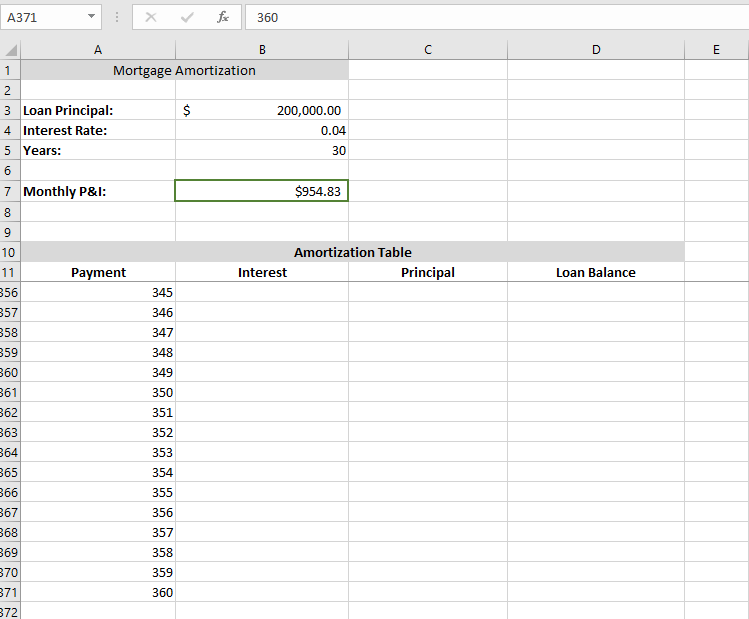
\includegraphics[width=0.75\textwidth]{ExcelAmortizationPaymentNumbers}
\end{center}

We'll carefully fill in the first two rows of the table, then use this functionality to drag the formulas down and generate the rest.
\vfill
\pagebreak

The interest for each month will be calculated by multiplying the balance at the end of the previous month by the interest rate divided by 12.  For the first row, we'll reference the starting balance (\$200,000) but after that, we want this calculation to reference the entry in column D and the previous row.
\begin{center}
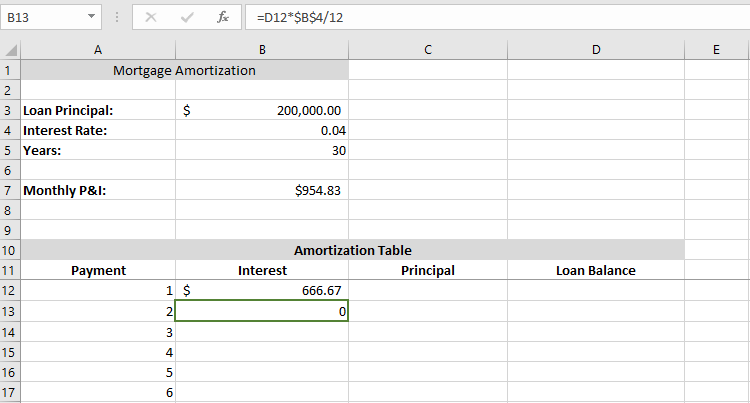
\includegraphics[width=0.75\textwidth]{ExcelAmortizationInterestCalculation}
\end{center}

\paragraph{What's with the dollar signs in B4?} Notice that instead of using B4 in the interest calculation, we are using \$B\$4.  The reason for this is that as we drag our formula down, Excel assumes that we want all of the cells in our formula to move in the same way.  This is, in fact, what we want to happen with the D12 in the formula; the next row should use D13, and so on.  To tell Excel to keep using the value in B4 even as we drag the formula down, you need to use these dollar signs.  You can insert them manually, or press F4 after clicking on the cell number in the formula.\\

The last two calculations are the principal and the loan balance: the principal payment will be the total monthly payment (\$B\$7) minus the interest payment, and the loan balance will be the previous balance minus the principal payment for the current month.
\begin{center}
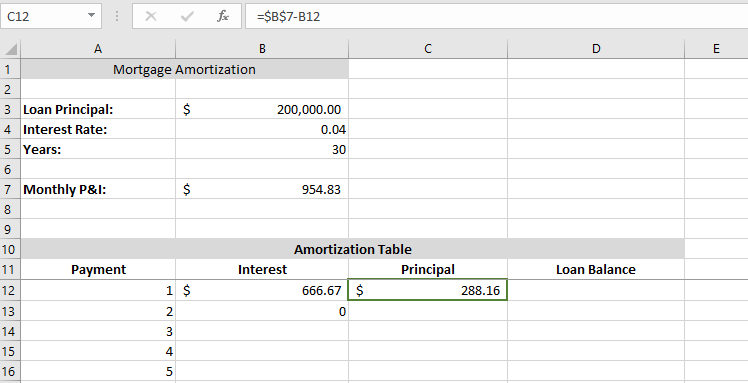
\includegraphics[width=0.75\textwidth]{ExcelAmortizationPrincipalCalculation}
\end{center}

After filling out the first two rows, you should have the following.  Notice that we did the first two rows manually because the first row uses the starting balance several times, which is not consistent with the formula we want to copy.
\begin{center}
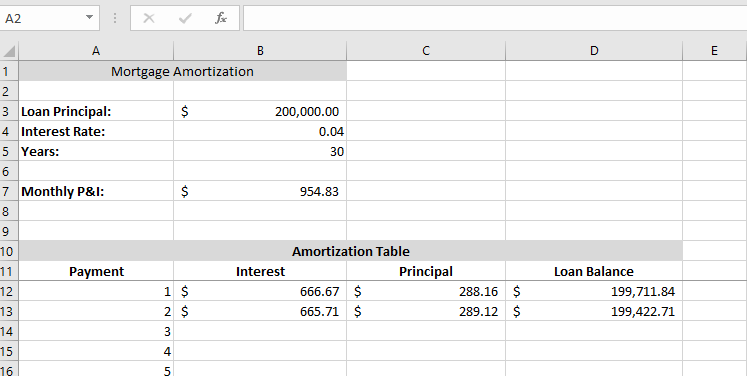
\includegraphics[width=0.75\textwidth]{ExcelAmortizationFirstTwoRows}
\end{center}
\pagebreak

The formulas we want to copy down are the ones in the second row (cells B13 through D13), so if we select those cells and drag downward all the way to payment 360, we'll get the full table:
\begin{center}
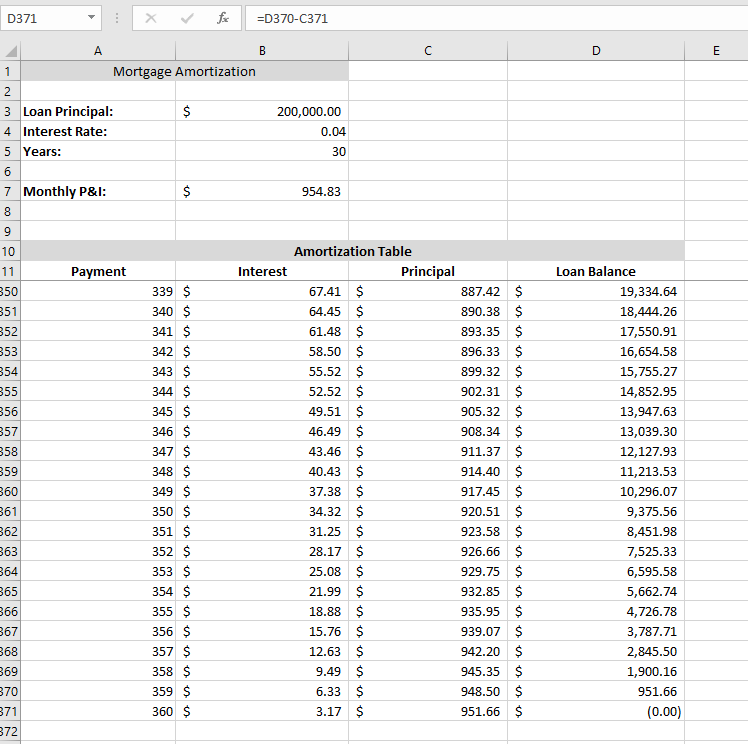
\includegraphics[width=0.75\textwidth]{ExcelAmortizationFullTable}
\end{center}

This shows the end of the table, where the loan balance finally drops to \$0.00.

\subsection{Credit Cards}
So far, we've dealt with \textit{fixed installment loans}, meaning that a specified amount is loaned and paid back with fixed payments in such a way that the balance goes to zero with the final scheduled payment.

On the other hand, there are \textbf{open-ended installment loans}, which require a variable payment each month, and the loan has no guaranteed end date; payments are made for as long as necessary to pay off the loan.  The most common example is a credit card, where the total balance does not have to be paid off each month, and any unpaid balance rolls over to the following month.  Of course, credit card companies take advantage of the ease of payment to rack up huge interest charges---credit card interest rates are among the highest you'll likely see.  If, on the other hand, you pay off the entire balance each month, treating the card more like a debit card, you'll never pay any interest charges to your credit card company.
\begin{center}
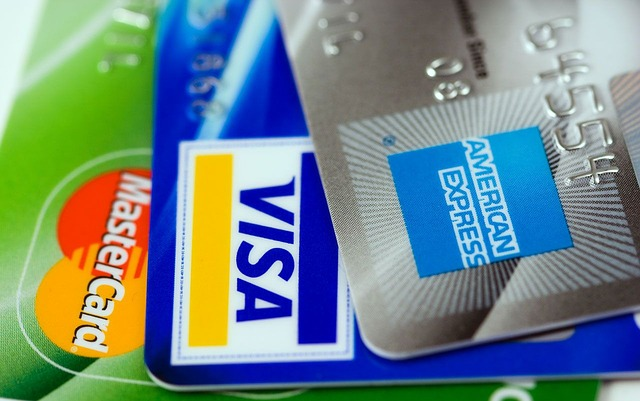
\includegraphics[scale=0.25]{CreditCards1}
\end{center}

\paragraph{Average Daily Balance Method} Different credit card companies calculate interest in different ways, all using the simple interest formula ($I=Prt$).  The difference lies in how $P$ is calculated; since the balance is constantly changing all month, they need a way to combine this all into a single principal.  The method we'll illustrate is called the \textit{average daily balance method}, which as the name suggests, takes the average of the balance on each day of the month.  Thus, if the balance was \$100 on the first 15 days of the month and \$200 on the last 15 days, the average daily balance will be \$150.
\vfill
\pagebreak

To find the average daily balance, add up the balance for each day and divide by the number of days.  In practice, we'll use a table to simplify the calculations by multiplying each different balance by the number of days that the card carried that balance.

\begin{example}[https://www.youtube.com/watch?v=ZUEQu_e2TqY]{Credit Card Charges}
Suppose your VISA card calculates interest using the average daily balance method, and the monthly interest rate is 1.5\% (notice that this means that the nominal annual rate is $1.5\% \times 12 = 18\%$, which is not at all unusually high for a credit card).  The itemized billing for the month of December is shown below.
\begin{center}
\begin{tabular}{l l l}
Detail & Date & Amount\\
\hline
Unpaid balance & December 1 & \$1500\\
Payment received & December 4 & \$300\\
Groceries & December 8 & \$125\\
Gas & December 15 & \$45\\
Wendy's & December 22 & \$8.50\\
Last day of billing period & December 31 &\\
Payment Due Date & January 7 &\\
\end{tabular}
\end{center}

\begin{enumerate}[(a)]
\item Find the average daily balance.
\item Find the interest due for December.
\item Find the total balance owed on the last day of the billing period.
\item This credit card requires a \$15 minimum monthly payment or $1/36$ of the amount due, whichever is higher.  What is the minimum monthly payment due by January 7?
\end{enumerate}

\sol
\begin{enumerate}[(a)]
\item Find the average daily balance.

To do this, we'll build a table to keep track of the unpaid balance after each transaction, and how long that unpaid balance lasts.

\begin{center}
\begin{tabular}{l l}
Date & Unpaid Balance\\
\hline
December 1 & \$1500\\
December 4 & \$1200\\
December 8 & \$1325\\
December 15 & \$1370\\
December 22 & \$1378.50\\
\end{tabular}
\end{center}

Now calculate how many days each balance lasted and multiply the balance by the number of days it lasted; this lets us quickly add up the balance for each day so that we can find the average by dividing this by the number of days.
\begin{center}
\begin{tabular}{l l p{0.7in} p{1.5in}}
Date & Unpaid Balance & Number of Days & (Unpaid balance) $\times$ (Number of Days)\\
\hline
December 1 & \$1500 & 3 & \$4500\\
December 4 & \$1200 & 4 & \$4800\\
December 8 & \$1325 & 7 & \$9275\\
December 15 & \$1370 & 7 & \$9590\\
December 22 & \$1378.50 & 10 & \$13,785\\
\hline
\textbf{Total:} & & 31 & \$41,950
\end{tabular}
\end{center}

The average daily balance is then the sum of the daily balances divided by 31, the number of days in the billing period:
\[\dfrac{\$41,950}{31} = \boxed{\$1353.23}\]

\item Find the interest due for December.

Use the simple interest formula, noting that since the interest rate is given as a \textit{monthly} rate, $t=1$ since we're dealing with a single month:
\[I=Prt = (\$1353.23)(0.015)(1) = \boxed{\$20.30}\]

\item Find the total balance owed on the last day of the billing period.

This is the final balance plus the interest charges:
\[\$1378.50 + \$20.30 = \boxed{\$1398.80}\]

\item This credit card requires a \$15 minimum monthly payment or 1/36 of the amount due, whichever is higher.  What is the minimum monthly payment due by January 7?

Since 1.36 of the amount due is $\$1398.80/36 = \$38.86$, which is more than \$15, the minimum payment due will be $\boxed{\$38.86}$
\end{enumerate}
\end{example}

\begin{try}
Suppose your VISA card calculates interest using the average daily balance method, and the monthly interest rate is 1.8\%.  The itemized billing for the month of May is shown below.
\begin{center}
\begin{tabular}{l l l}
Detail & Date & Amount\\
\hline
Unpaid balance & May 1 & \$850\\
Payment received & May 5 & \$200\\
Groceries & May 7 & \$240\\
Gas & May 13 & \$33\\
Jewelry Store & May 25 & \$575\\
Last day of billing period & May 31 &\\
Payment Due Date & June 7 &\\
\end{tabular}
\end{center}

\begin{enumerate}[(a)]
\item Find the average daily balance.
\item Find the interest due for this month.
\item Find the total balance owed on the last day of the billing period.
\item This credit card requires a \$20 minimum payment or 1/24 of the amount due, whichever is higher.  What is the minimum monthly payment due for this month?
\end{enumerate}
\end{try}

We'll finish this discussion by taking another look at the trap of the minimum payment; we'll use the numbers from the preceding example.  A minimum payment of \$38.84 on a balance of \$1398.13 sounds pretty reasonable, but think about how long it would take to pay off this balance by only making the minimum payment each month (even without adding further charges), since the majority of the minimum payment will go toward interest.

Skipping over the details (this can be figured out using a simple spreadsheet), if you started with a balance of \$1398.13 and never added another charge, just making the minimum payment each month, it would take 123 months to pay it off, or over 10 years.  In doing so, you would end up paying a total of \$2571.46, or nearly twice what you owed.  The lesson is simple: pay off your credit card in full as much as possible, and don't live beyond your means in a way that requires the use of credit to get by.